\documentclass[12pt,a4paper]{article}
\usepackage[utf8]{vietnam}
\usepackage{amsmath,amssymb}
\usepackage{tabularx}
\usepackage{graphicx}
\usepackage{tikz}
\usetikzlibrary{calc,arrows.meta}
\usepackage{xcolor}
\usepackage{enumitem}
\usepackage{fancyhdr}
\usepackage[top=1.2cm, bottom=1.2cm, left=1.5cm, right=1.5cm]{geometry}
\usepackage[loigiai]{ex_test}
\SAOPTN{widthSA=2.6,heightSA=0.62}

\setlength{\headheight}{15pt}
\setlength{\parskip}{0pt}

\pagestyle{fancy}
\fancyhf{}
\rhead{\textit{Lời giải chi tiết -- Đề số 8}}
\lhead{\textit{Bộ đề ôn tập Giữa học kì I -- Toán 7}}
\cfoot{\thepage}

\begin{document}

\begin{center}
\textbf{\Large HƯỚNG DẪN CHẤM VÀ LỜI GIẢI CHI TIẾT}\\
\vspace{1.5mm}
\textbf{\large MÔN: TOÁN 7 -- ĐỀ SỐ 8}
\end{center}
\vspace{2mm}

\noindent\textbf{\large PHẦN I. CÂU TRẮC NGHIỆM NHIỀU PHƯƠNG ÁN LỰA CHỌN}

\vspace{1mm}
\begin{ex}
Số nào dưới đây là số hữu tỉ dương?
\choice
{\True $\dfrac{-3}{-2}$}
{$-\dfrac{2}{7}$}
{$-\dfrac{1}{3}$}
{$-\dfrac{3}{15}$}
\loigiai{
Ta có $\dfrac{-3}{-2} = \dfrac{3}{2} > 0$ nên là số hữu tỉ dương. Các số còn lại đều nhỏ hơn $0$.
}
\end{ex}

\begin{ex}
Căn bậc hai số học của $64$ là:
\choice
{$32$}
{$8$ và $-8$}
{$-8$}
{\True $8$}
\loigiai{
Căn bậc hai số học của số $a \ge 0$ là số không âm $\sqrt{a}$. Do $8 > 0$ và $8^2 = 64$ nên căn bậc hai số học của $64$ là $8$.
}
\end{ex}

\begin{ex}
\immini{
Quan sát trục số sau. Điểm $a$ biểu diễn số hữu tỉ nào?
\choice
{$a = \dfrac{1}{3}$}
{$a = 2\dfrac{1}{3}$}
{$a = 1\dfrac{2}{3}$}
{\True $a = \dfrac{2}{3}$}
}{
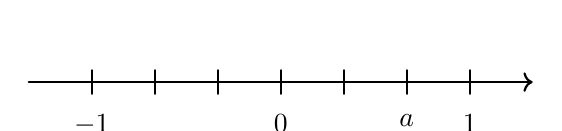
\begin{tikzpicture}[scale=1.0, line cap=round, line join=round]
    \draw[thick, ->] (-3.2, 0) -- (3.2, 0);
    \foreach \x/\label in {-2.4/-1, -1.6/{}, -0.8/{}, 0/0, 0.8/{}, 1.6/a, 2.4/1} {
        \draw[thick] (\x, 0.15) -- (\x, -0.15);
        \ifx\label\empty\else
            \node[below=4pt] at (\x, -0.15) {$\label$};
        \fi
    }
\end{tikzpicture}
}
\loigiai{
Đoạn thẳng đơn vị từ $0$ đến $1$ được chia thành $3$ phần bằng nhau, mỗi phần ứng với $\dfrac{1}{3}$. Điểm $a$ nằm ở vạch thứ hai bên phải điểm $0$, do đó $a = \dfrac{2}{3}$.
}
\end{ex}

\begin{ex}
Trong các hình sau, hình nào có dạng là hình lăng trụ đứng tam giác?
\begin{center}
\begin{tabular}{cccc}
\includegraphics[height=1.5cm]{crops/test_p35_xref2563.png} &
\includegraphics[height=1.5cm]{crops/test_p35_xref2564.jpeg} &
\includegraphics[height=1.5cm]{crops/test_p35_xref2565.jpeg} &
\includegraphics[height=1.5cm]{crops/test_p35_xref2566.jpeg} \\
\textbf{Hình 1} & \textbf{Hình 2} & \textbf{Hình 3} & \textbf{Hình 4}
\end{tabular}
\end{center}
\choice
{Hình 1}
{Hình 2}
{Hình 3}
{\True Hình 4}
\loigiai{
Hình 1 là hình lăng trụ đứng lục giác; Hình 2 là hình trụ; Hình 3 là hình hộp chữ nhật; Hình 4 có hai mặt đáy là tam giác và các mặt bên là hình chữ nhật nên là hình lăng trụ đứng tam giác.
}
\end{ex}

\begin{ex}
\immini{
Hai đường thẳng $AB$ và $CD$ cắt nhau tại $O$. Góc đối đỉnh với $\widehat{AOC}$ là:
\choice
{$\widehat{AOC}$}
{$\widehat{AOD}$}
{\True $\widehat{DOB}$}
{$\widehat{BOC}$}
}{
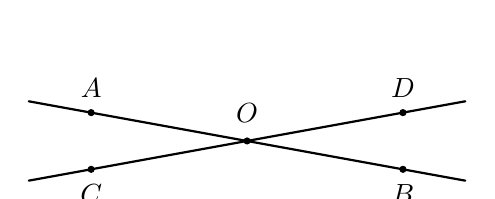
\begin{tikzpicture}[scale=0.9, line cap=round, line join=round]
    \coordinate (O) at (0, 0);
    \coordinate (A) at (-2.2, 0.4);
    \coordinate (B) at (2.2, -0.4);
    \coordinate (C) at (-2.2, -0.4);
    \coordinate (D) at (2.2, 0.4);

    \draw[thick] ($(A)!-0.2!(B)$) -- ($(B)!-0.2!(A)$);
    \draw[thick] ($(C)!-0.2!(D)$) -- ($(D)!-0.2!(C)$);

    \filldraw[black] (A) circle (1.2pt) node[above=2pt] {$A$};
    \filldraw[black] (B) circle (1.2pt) node[below=2pt] {$B$};
    \filldraw[black] (C) circle (1.2pt) node[below=2pt] {$C$};
    \filldraw[black] (D) circle (1.2pt) node[above=2pt] {$D$};
    \filldraw[black] (O) circle (1.2pt) node[above=3pt] {$O$};
\end{tikzpicture}
}
\loigiai{
Hai đường thẳng $AB$ và $CD$ cắt nhau tại $O$. Tia $OB$ đối với tia $OA$, tia $OD$ đối với tia $OC$. Do đó góc đối đỉnh với $\widehat{AOC}$ là $\widehat{DOB}$ (hay $\widehat{BOD}$).
}
\end{ex}

\begin{ex}
Kết quả của phép nhân $(0{,}25)^8 \cdot (0{,}25)^4$ là:
\choice
{\True $(0{,}25)^{12}$}
{$(0{,}25)^4$}
{$(0{,}25)^2$}
{$(0{,}25)^{32}$}
\loigiai{
Áp dụng quy tắc nhân hai lũy thừa cùng cơ số: $(0{,}25)^8 \cdot (0{,}25)^4 = (0{,}25)^{8+4} = (0{,}25)^{12}$.
}
\end{ex}

\begin{ex}
Khẳng định nào sau đây là đúng?
\choice
{Nếu $a$ là số tự nhiên thì $a$ là số vô tỉ}
{\True Nếu $a$ là số hữu tỉ thì $a$ không thể là số vô tỉ}
{Số thập phân vô hạn tuần hoàn là số vô tỉ}
{Số thập phân hữu hạn là số vô tỉ}
\loigiai{
Tập hợp số hữu tỉ $\mathbb{Q}$ và tập hợp số vô tỉ $\mathbb{I}$ là hai tập hợp rời nhau: $\mathbb{Q} \cap \mathbb{I} = \emptyset$. Do đó, nếu $a$ là số hữu tỉ thì $a$ không thể là số vô tỉ.
}
\end{ex}

\begin{ex}
Trong các số sau, số nào là số vô tỉ?
\choice
{$5^2$}
{\True $\sqrt{3}$}
{$(3{,}5)^2$}
{$16$}
\loigiai{
Ta có $5^2 = 25$, $(3{,}5)^2 = 12{,}25$, $16$ đều là các số hữu tỉ. Số $\sqrt{3} \approx 1{,}73205\dots$ là số thập phân vô hạn không tuần hoàn nên là số vô tỉ.
}
\end{ex}

\begin{ex}
Cho tam giác $ABC$ có $\widehat{A} = 70^\circ, \widehat{B} = 50^\circ$. Số đo góc $C$ là:
\choice
{\True $60^\circ$}
{$70^\circ$}
{$80^\circ$}
{$90^\circ$}
\loigiai{
Tổng ba góc trong một tam giác bằng $180^\circ$. Do đó:
\[ \widehat{C} = 180^\circ - (\widehat{A} + \widehat{B}) = 180^\circ - (70^\circ + 50^\circ) = 60^\circ. \]
}
\end{ex}

\begin{ex}
Bạn Việt tiết kiệm được $105\,000$ đồng. Nhằm thực hiện thông điệp 5K chủ động phòng chống dịch Covid-19, bạn Việt đã dùng $\dfrac{1}{3}$ số tiền tiết kiệm được để mua khẩu trang. Bạn Việt còn lại bao nhiêu tiền?
\choice
{$25\,000$ đồng}
{$30\,000$ đồng}
{$35\,000$ đồng}
{\True $70\,000$ đồng}
\loigiai{
Số tiền bạn Việt dùng để mua khẩu trang là:
\[ 105\,000 \cdot \dfrac{1}{3} = 35\,000\text{ (đồng)}. \]
Số tiền bạn Việt còn lại là:
\[ 105\,000 - 35\,000 = 70\,000\text{ (đồng)}. \]
}
\end{ex}

\begin{ex}
Tìm số nguyên $a$ để $-\dfrac{3}{4} < \dfrac{a}{10} < -\dfrac{3}{5}$:
\choice
{$a \in \{-6; -7\}$}
{$a = -6$}
{\True $a = -7$}
{$a \in \{-7; -8\}$}
\loigiai{
Quy đồng mẫu số chung là $20$:
\[ -\dfrac{15}{20} < \dfrac{2a}{20} < -\dfrac{12}{20} \implies -15 < 2a < -12. \]
Vì $a \in \mathbb{Z}$ nên $2a$ là số nguyên chẵn nằm giữa $-15$ và $-12$. Do đó $2a = -14 \implies a = -7$.
}
\end{ex}

\begin{ex}
Cho hình lăng trụ đứng tam giác $ABC.A'B'C'$. Các mặt bên của hình lăng trụ trên là những hình gì?
\choice
{Hình tam giác}
{Hình tứ giác}
{\True Hình chữ nhật}
{Hình vuông}
\loigiai{
Theo định nghĩa hình lăng trụ đứng, các mặt bên của hình lăng trụ đứng luôn là các hình chữ nhật.
}
\end{ex}


\setcounter{ex}{0}
\noindent\textbf{\large PHẦN II. CÂU TRẮC NGHIỆM ĐÚNG SAI}

\vspace{1mm}
\begin{ex}
Cho hai biểu thức $A = \left(-\dfrac{1}{3}\right)^2 \cdot 9 - \left|-\dfrac{5}{2}\right|$ và $B = \dfrac{7}{4} : \left(-\dfrac{1}{2}\right)$. Xét tính đúng sai của các mệnh đề sau:
\choiceTF
{\True Giá trị của lũy thừa $\left(-\dfrac{1}{3}\right)^2$ bằng $\dfrac{1}{9}$}
{\True Giá trị của biểu thức $A$ bằng $-\dfrac{3}{2}$}
{Kết quả của phép tính $B = \dfrac{7}{4} : \left(-\dfrac{1}{2}\right)$ bằng $-\dfrac{7}{8}$}
{\True Tổng $A + B$ có giá trị bằng $-5$}
\loigiai{
\begin{itemize}[leftmargin=0.5cm, itemsep=1pt]
\item \textbf{a)} \textbf{Đúng}. Ta có $\left(-\dfrac{1}{3}\right)^2 = \dfrac{(-1)^2}{3^2} = \dfrac{1}{9}$.
\item \textbf{b)} \textbf{Đúng}. Ta có $A = \dfrac{1}{9} \cdot 9 - \dfrac{5}{2} = 1 - \dfrac{5}{2} = -\dfrac{3}{2}$.
\item \textbf{c)} \textbf{Sai}. Ta có $B = \dfrac{7}{4} \cdot (-2) = -\dfrac{7}{2} \neq -\dfrac{7}{8}$.
\item \textbf{d)} \textbf{Đúng}. Ta có $A + B = -\dfrac{3}{2} + \left(-\dfrac{7}{2}\right) = -\dfrac{10}{2} = -5$.
\end{itemize}
}
\end{ex}

\begin{ex}
\immini{
Quan sát hình vẽ, biết $\widehat{CFE} = 55^\circ$ và $\widehat{E}_1 = 125^\circ$. Xét tính đúng sai của các mệnh đề sau:
\choiceTF
{\True Góc $\widehat{AEF}$ và góc $\widehat{E}_1$ là hai góc đối đỉnh}
{\True Số đo của góc $\widehat{FEB}$ bằng $55^\circ$}
{\True Hai đường thẳng $CD$ và $AB$ song song với nhau}
{Số đo của góc $\widehat{EFD}$ bằng $110^\circ$}
}{
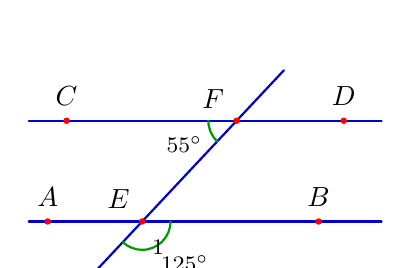
\begin{tikzpicture}[scale=0.8, line cap=round, line join=round]
    \coordinate (E) at (1.0, 0);
    \coordinate (F) at (2.5, 1.6);

    \draw[thick, blue!80!black] (-0.8, 1.6) -- (4.8, 1.6);
    \draw[thick, blue!80!black] (-0.8, 0) -- (4.8, 0);

    \filldraw[red] (-0.2, 1.6) circle (1.2pt) node[above=2pt, black] {$C$};
    \filldraw[red] (4.2, 1.6) circle (1.2pt) node[above=2pt, black] {$D$};
    \filldraw[red] (-0.5, 0) circle (1.2pt) node[above=2pt, black] {$A$};
    \filldraw[red] (3.8, 0) circle (1.2pt) node[above=2pt, black] {$B$};

    \draw[thick, blue!80!black] ($(E)!-0.5!(F)$) -- ($(F)!-0.5!(E)$);

    \filldraw[red] (E) circle (1.2pt) node[above left=1pt, black] {$E$};
    \filldraw[red] (F) circle (1.2pt) node[above left=1pt, black] {$F$};

    \draw[green!60!black, thick] (F) ++(180:0.45) arc (180:227:0.45);
    \node[font=\footnotesize, below left=1pt] at ($(F)+(-0.35, -0.05)$) {$55^\circ$};

    \draw[green!60!black, thick] (E) ++(0:0.45) arc (0:-133:0.45);
    \node[font=\footnotesize, below=2pt] at ($(E)+(0.25, -0.05)$) {$1$};
    \node[font=\footnotesize, below right=1pt] at ($(E)+(0.1, -0.35)$) {$125^\circ$};
\end{tikzpicture}
}
\loigiai{
\begin{itemize}[leftmargin=0.5cm, itemsep=1pt]
\item \textbf{a)} \textbf{Đúng}. Tia $EA$ đối với tia $EB$, tia $EF$ đối với tia đối của nó tạo thành hai góc đối đỉnh $\widehat{AEF}$ và $\widehat{E}_1$.
\item \textbf{b)} \textbf{Đúng}. Vì $\widehat{FEB}$ và $\widehat{E}_1$ là hai góc kề bù nên $\widehat{FEB} = 180^\circ - 125^\circ = 55^\circ$.
\item \textbf{c)} \textbf{Đúng}. Ta có $\widehat{CFE} = \widehat{FEB} = 55^\circ$. Mà hai góc này ở vị trí so le trong nên $CD \parallel AB$.
\item \textbf{d)} \textbf{Sai}. Vì $\widehat{EFD}$ và $\widehat{CFE}$ là hai góc kề bù nên $\widehat{EFD} = 180^\circ - 55^\circ = 125^\circ \neq 110^\circ$.
\end{itemize}
}
\end{ex}


\setcounter{ex}{0}
\noindent\textbf{\large PHẦN III. CÂU HỎI TRẢ LỜI NGẮN}

\vspace{1mm}
\begin{ex}
Tính giá trị của biểu thức: $A = \dfrac{15^3 \cdot 2^4}{6^3 \cdot 5^2}$. \shortans{$10$}
\loigiai{
Phân tích ra thừa số nguyên tố:
\[ A = \dfrac{(3 \cdot 5)^3 \cdot 2^4}{(2 \cdot 3)^3 \cdot 5^2} = \dfrac{3^3 \cdot 5^3 \cdot 2^4}{2^3 \cdot 3^3 \cdot 5^2} = 2^{4-3} \cdot 3^{3-3} \cdot 5^{3-2} = 2 \cdot 1 \cdot 5 = 10. \]
}
\end{ex}

\begin{ex}
\immini{
Cho hình vẽ sau, biết $a \parallel b, \widehat{A}_4 = 135^\circ$. Số đo của $\widehat{B}_2$ bằng bao nhiêu độ?
\vspace{1mm}
\hfill\shortans{$135^\circ$}
}{
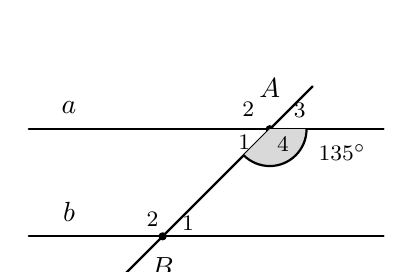
\begin{tikzpicture}[scale=0.85, line cap=round, line join=round]
    \coordinate (B) at (1.2, 0);
    \coordinate (A) at (2.8, 1.6);

    \draw[thick] (-0.8, 1.6) -- (4.5, 1.6);
    \node[above=2pt] at (-0.2, 1.6) {$a$};
    \draw[thick] (-0.8, 0) -- (4.5, 0);
    \node[above=2pt] at (-0.2, 0) {$b$};

    \draw[thick] ($(A)!1.4!(B)$) -- ($(B)!1.4!(A)$);

    \filldraw[black] (A) circle (1.5pt) node[above=8pt] {$A$};
    \filldraw[black] (B) circle (1.5pt) node[below=4pt] {$B$};

    \fill[gray!30] (A) -- ++(0:0.55) arc (0:-135:0.55) -- cycle;
    \draw[thick] (A) ++(0:0.55) arc (0:-135:0.55);
    \node[font=\footnotesize] at ($(A)+(0.2, -0.22)$) {$4$};
    \node[font=\footnotesize, right=2pt] at ($(A)+(0.5, -0.35)$) {$135^\circ$};

    \node[font=\footnotesize] at ($(A)+(-0.38, -0.2)$) {$1$};
    \node[font=\footnotesize] at ($(A)+(-0.32, 0.3)$) {$2$};
    \node[font=\footnotesize] at ($(A)+(0.45, 0.28)$) {$3$};

    \node[font=\footnotesize] at ($(B)+(0.38, 0.2)$) {$1$};
    \node[font=\footnotesize] at ($(B)+(-0.15, 0.25)$) {$2$};
\end{tikzpicture}
}
\loigiai{
Vì $a \parallel b$ nên hai góc so le trong bằng nhau: $\widehat{B}_2 = \widehat{A}_4 = 135^\circ$.
}
\end{ex}


\setcounter{ex}{0}
\noindent\textbf{\large PHẦN IV. TỰ LUẬN}

\vspace{1mm}
\begin{ex}
Thực hiện phép tính (tính hợp lí nếu có):
\begin{enumerate}[label=\textbf{\alph*)}, leftmargin=0.8cm, itemsep=1pt]
\item $\dfrac{5}{2} + 0{,}75$;
\item $-\dfrac{2}{11} + \dfrac{3}{5} - \dfrac{9}{11} + \dfrac{2}{5} + 2025$;
\item $-\dfrac{1}{13} \cdot \dfrac{5}{18} + \left(-\dfrac{1}{13}\right) \cdot \dfrac{13}{18} + \dfrac{(-1)^{2026}}{13}$.
\end{enumerate}
\loigiai{
\textbf{a)} \[ \dfrac{5}{2} + 0{,}75 = 2{,}5 + 0{,}75 = 3{,}25 = \dfrac{13}{4}. \]

\textbf{b)} \[ \begin{aligned} -\dfrac{2}{11} + \dfrac{3}{5} - \dfrac{9}{11} + \dfrac{2}{5} + 2025 &= \left(-\dfrac{2}{11} - \dfrac{9}{11}\right) + \left(\dfrac{3}{5} + \dfrac{2}{5}\right) + 2025 \\ &= -1 + 1 + 2025 = 2025. \end{aligned} \]

\textbf{c)} \[ \begin{aligned} -\dfrac{1}{13} \cdot \dfrac{5}{18} + \left(-\dfrac{1}{13}\right) \cdot \dfrac{13}{18} + \dfrac{(-1)^{2026}}{13} &= -\dfrac{1}{13} \cdot \left(\dfrac{5}{18} + \dfrac{13}{18}\right) + \dfrac{1}{13} \\ &= -\dfrac{1}{13} \cdot 1 + \dfrac{1}{13} = 0. \end{aligned} \]

}
\end{ex}
\vspace{1.5mm}

\begin{ex}
Cho các số sau: $3{,}9;\ 29\%;\ \sqrt{7};\ 0{,}(8);\ -\dfrac{4}{99};\ \pi;\ -\sqrt{5};\ 3$. Trong các số trên, có bao nhiêu số vô tỉ?
\loigiai{
Ta phân loại các số đã cho:
- Các số hữu tỉ: $3{,}9 = \dfrac{39}{10}$; $29\% = \dfrac{29}{100}$; $0{,}(8) = \dfrac{8}{9}$; $-\dfrac{4}{99}$; $3 = \dfrac{3}{1}$.
- Các số vô tỉ: $\sqrt{7}$; $\pi$; $-\sqrt{5}$. (Lưu ý: trong đề nếu có $4$ số vô tỉ là $\sqrt{7}, \pi, -\sqrt{5}$ và số thứ 4 nếu có căn).
Vậy trong các số trên có $3$ (hoặc $4$) số vô tỉ.
}
\end{ex}
\vspace{1.5mm}

\begin{ex}
\immini{
Cho hình vẽ, biết $\widehat{ABI} = 80^\circ$.
\begin{enumerate}[label=\textbf{\alph*)}, leftmargin=0.8cm, itemsep=1pt]
\item Chứng minh $m \parallel n$.
\item Tính số đo $\widehat{cAH}$ và $\widehat{mAc}$.
\item Vẽ tia $AE$ là tia phân giác của $\widehat{cAH}$, tia $BF$ là tia phân giác của $\widehat{ABI}$. Chứng minh $AE \parallel BF$.
\end{enumerate}
}{
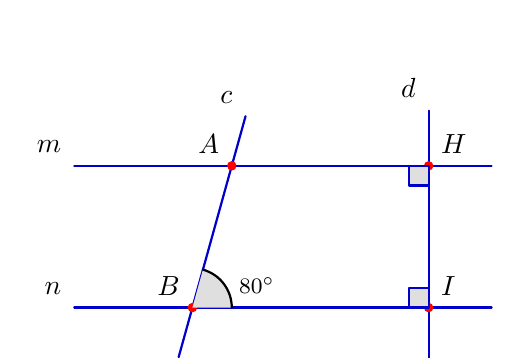
\begin{tikzpicture}[scale=1.0, line cap=round, line join=round]
    \draw[thick, blue!80!black] (-0.5, 1.8) node[above left=1pt, black] {$m$} -- (4.8, 1.8);
    \draw[thick, blue!80!black] (-0.5, 0) node[above left=1pt, black] {$n$} -- (4.8, 0);

    \coordinate (B) at (1.0, 0);
    \coordinate (A) at (1.5, 1.8);
    \coordinate (I) at (4.0, 0);
    \coordinate (H) at (4.0, 1.8);

    \draw[thick, blue!80!black] ($(B)!1.35!(A)$) node[above left=1pt, black] {$c$} -- ($(A)!1.35!(B)$);
    \draw[thick, blue!80!black] ($(I)+(0, 2.5)$) node[above left=1pt, black] {$d$} -- ($(I)+(0, -0.8)$);

    \filldraw[red] (A) circle (1.5pt) node[above left=1pt, black] {$A$};
    \filldraw[red] (B) circle (1.5pt) node[above left=1pt, black] {$B$};
    \filldraw[red] (H) circle (1.5pt) node[above right=1pt, black] {$H$};
    \filldraw[red] (I) circle (1.5pt) node[above right=1pt, black] {$I$};

    \draw[thick, blue!80!black, fill=gray!25] (H) rectangle +(-0.25, -0.25);
    \draw[thick, blue!80!black, fill=gray!25] (I) rectangle +(-0.25, 0.25);

    \fill[gray!25] (B) -- ++(0:0.5) arc (0:74.5:0.5) -- cycle;
    \draw[thick] (B) ++(0:0.5) arc (0:74.5:0.5);
    \node[font=\footnotesize, right=2pt] at ($(B)+(0.4, 0.28)$) {$80^\circ$};
\end{tikzpicture}
}
\loigiai{
\textbf{a)} Theo hình vẽ, ta có $d \perp m$ tại $H$ và $d \perp n$ tại $I$.
Hai đường thẳng $m$ và $n$ phân biệt cùng vuông góc với đường thẳng $d$ nên $m \parallel n$.

\textbf{b)} Vì $m \parallel n$ nên $\widehat{cAH} = \widehat{ABI} = 80^\circ$ (hai góc đồng vị).
Vì $\widehat{mAc}$ và $\widehat{cAH}$ là hai góc kề bù nên:
\[ \widehat{mAc} + \widehat{cAH} = 180^\circ \implies \widehat{mAc} = 180^\circ - 80^\circ = 100^\circ. \]

\textbf{c)} Vì $AE$ là tia phân giác của $\widehat{cAH}$ nên $\widehat{cAE} = \dfrac{1}{2}\widehat{cAH} = \dfrac{1}{2} \cdot 80^\circ = 40^\circ$.
Vì $BF$ là tia phân giác của $\widehat{ABI}$ nên $\widehat{ABF} = \dfrac{1}{2}\widehat{ABI} = \dfrac{1}{2} \cdot 80^\circ = 40^\circ$.
Suy ra $\widehat{cAE} = \widehat{ABF} = 40^\circ$.
Mà hai góc này ở vị trí đồng vị nên $AE \parallel BF$.

}
\end{ex}
\vspace{1.5mm}

\begin{ex}
Một cửa hàng nhập về $100$ cái áo với giá gốc $200\,000$ đồng/cái. Cửa hàng đã bán $60$ cái áo với giá mỗi cái lãi $25\%$ so với giá gốc, $40$ cái còn lại bán lỗ $10\%$ so với giá gốc. Hỏi sau khi bán hết $100$ cái áo, cửa hàng đó lãi hay lỗ bao nhiêu tiền?
\loigiai{
Tổng chi phí nhập $100$ cái áo là:
\[ 100 \cdot 200\,000 = 20\,000\,000\text{ (đồng)}. \]
Số tiền lãi từ mỗi cái áo trong $60$ cái đầu là:
\[ 200\,000 \cdot 25\% = 50\,000\text{ (đồng)}. \]
Tổng số tiền lãi từ $60$ cái áo là:
\[ 60 \cdot 50\,000 = 3\,000\,000\text{ (đồng)}. \]
Số tiền lỗ từ mỗi cái áo trong $40$ cái còn lại là:
\[ 200\,000 \cdot 10\% = 20\,000\text{ (đồng)}. \]
Tổng số tiền lỗ từ $40$ cái áo là:
\[ 40 \cdot 20\,000 = 800\,000\text{ (đồng)}. \]
Vì số tiền lãi lớn hơn số tiền lỗ nên sau khi bán hết $100$ cái áo, cửa hàng có lãi. Số tiền lãi là:
\[ 3\,000\,000 - 800\,000 = 2\,200\,000\text{ (đồng)}. \]
Đáp số: Cửa hàng lãi $2\,200\,000$ đồng.
}
\end{ex}
\vspace{1.5mm}


\begin{center}
\rule{4cm}{0.4pt}\\
\textit{--- HẾT ---}
\end{center}
\end{document}
